
% Backup of latexcode.tex
% Created on 2025-12-10

\documentclass[11pt]{article}

% -------------------- Page & Layout --------------------
\usepackage[margin=1in]{geometry}

% -------------------- Math Packages --------------------
\usepackage{amsmath, amssymb, amsthm}
\usepackage{mathtools}

% -------------------- Graphics & Figures --------------------
\usepackage{tikz}

\usepackage{graphicx}
\usepackage{pgfplots}
\pgfplotsset{compat=1.18}

% -------------------- Tables --------------------
\usepackage{array}
\usepackage{booktabs}

% -------------------- Misc --------------------
\usepackage{enumitem}   % better control of lists
\usepackage[colorlinks=true,linkcolor=blue,citecolor=blue,urlcolor=blue]{hyperref}

% -------------------- Theorem Styles --------------------
\newtheoremstyle{spaced}%
	{10pt}   % Space above
	{10pt}   % Space below
	{\itshape} % Body font
	{}       % Indent amount
	{\bfseries} % Theorem head font
	{.}      % Punctuation after theorem head
	{0.5em}  % Spa ce after theorem head
	{}       % Theorem head spec

	heoremstyle{spaced}
\newtheorem{theorem}{Theorem}[section]
\newtheorem{lemma}[theorem]{Lemma}
\newtheorem{proposition}[theorem]{Proposition}
\newtheorem{corollary}[theorem]{Corollary}

	heoremstyle{definition}
\newtheorem{definition}[theorem]{Definition}

	heoremstyle{remark}
\newtheorem{remark}[theorem]{Remark}
\newtheorem{example}[theorem]{Example}

% -------------------- Title Info --------------------
	itle{Track Layouts, Forbidden Patterns, and Degree Bounds}
\author{Axel Fridman}

% =====================================================
\begin{document}
% =====================================================

\maketitle

\begin{abstract}
We study ordered layouts of a graph on $k$ ``tracks'' in which edges are 
constrained by nearest-neighbor rules. This notion comes from the Investigathon
formulation in terms of forbidden colored patterns on triples of vertices.
We make the correspondence between the two formalisms precise, define
\emph{$k$-track triplet-legal layouts}, and then investigate how many tracks
(i.e., ``colors'') are necessary for a given graph. We prove degree bounds,
planarity results for $k \le 2$, and structural examples such as cycles and
graphs obtained from a path by adding one extra edge. Along the way we
highlight exactly when $k<=2$ (``less than three colors'') is possible.
\end{abstract}

	ableofcontents

% =====================================================
\section{Basic Setup: Tracks, Order, and Legal Neighbors}
% =====================================================
\label{sec:basic-setup}
Throughout, $G=(V,E)$ is a finite simple undirected graph.

\subsection{Ordered $k$-track layouts}

We begin with the purely combinatorial structure of tracks and a global order.

\begin{definition}[Ordered $k$-track layout]
Let $k\in\mathbb{N}$. A \emph{$k$-track ordered layout} of a graph $G=(V,E)$ is a pair
\[
	(\tau,p)
\]
consisting of
\begin{itemize}[leftmargin=2em]
	\item a \emph{track assignment}
	\[
			au : V \to \{1,\dots,k\},
	\]
	\item and a bijective \emph{position map}
	\[
		p : V \to \{1,\dots,|V|\}.
	\]
\end{itemize}
We write $x<y$ if and only if $p(x) < p(y)$ and think of all vertices laid out
from left to right according to $p$.
\end{definition} 
An example is shown in Figure~\ref{fig:tracks-basic}.
\begin{figure}[ht]
	\centering
	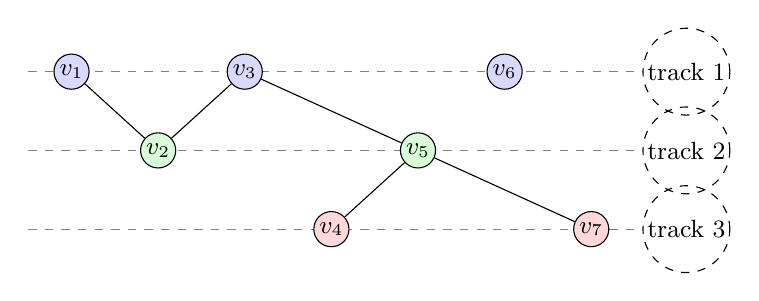
\begin{tikzpicture}[x=1.1cm,y=1cm,
		every node/.style={circle,draw,inner sep=1pt,font=\small}]
		% Track lines
		\foreach \t/\y in {1/2.0,2/1.0,3/0.0} {
			\draw[dashed,gray] (0.5,\y) -- (7.5,\y)
				node[right=1mm,black] {$\text{track }\t$};
		}

		% Vertices in global order (p(v_i) = i)
		\node[fill=blue!15]  (v1) at (1,2.0) {$v_1$};
		\node[fill=green!15] (v2) at (2,1.0) {$v_2$};
		\node[fill=blue!15]  (v3) at (3,2.0) {$v_3$};
		\node[fill=red!15]   (v4) at (4,0.0) {$v_4$};
		\node[fill=green!15] (v5) at (5,1.0) {$v_5$};
		\node[fill=blue!15]  (v6) at (6,2.0) {$v_6$};
		\node[fill=red!15]   (v7) at (7,0.0) {$v_7$};

		% Sample edges
		\draw (v1) -- (v2);
		\draw (v2) -- (v3);
		\draw (v3) -- (v5);
		\draw (v4) -- (v5);
		\draw (v5) -- (v7);
	\end{tikzpicture}
	\caption{An example of a $3$-track ordered layout: global order is left-to-right, colors indicate the track assignment $\tau$.}
	\label{fig:tracks-basic}
\end{figure}

For each track $t\in\{1,\dots,k\}$ we define the vertex set
\[
	V_t := \{v\in V : \tau(v) = t\},
\]
ordered by increasing $p(\cdot)$ along that track.

\begin{definition}[Predecessor, successor on a track]
Given a $k$-track layout $(\tau,p)$, a vertex $v\in V$, and a track $t$,
we define:
\begin{align*}
	\operatorname{pred}_t(v) 
	&:= \text{the vertex in $V_t$ with largest $p(\cdot)$ strictly less than $p(v)$ (if it exists)},\\
	\operatorname{succ}_t(v) 
	&:= \text{the vertex in $V_t$ with smallest $p(\cdot)$ strictly greater than $p(v)$ (if it exists)}.
\end{align*}
If such a vertex does not exist, the predecessor/successor is said to be
``nonexistent.'' Intuitively, these are the nearest neighbors of $v$ on track $t$
to the left/right in the global order.
\end{definition} 
See Figure~\ref{fig:predsucc} for a pictorial view along a single track.
\par\vspace{1em}


\begin{figure}[ht]
	\centering
	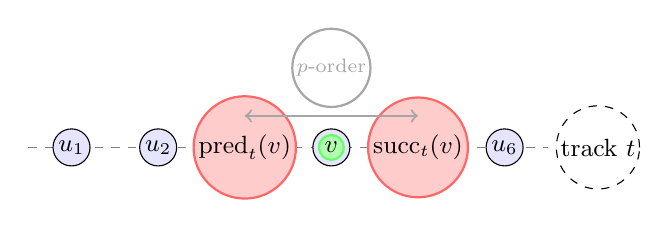
\begin{tikzpicture}[x=1.1cm,y=1cm,
		every node/.style={circle,draw,inner sep=1pt,font=\small}]
		% Single track line
		\draw[dashed,gray] (0.5,0) -- (6.5,0)
			node[right=1mm,black] {$\text{track }t$};

		% Vertices on track t
		\foreach \i in {1,...,6} {
			\node[fill=blue!10] (u\i) at (\i,0) {$u_{\i}$};
		}

		% Highlight v = u4
		\node[fill=green!30,draw=green!60,thick] (v) at (4,0) {$v$};

		% Overwrite labels for pred and succ
		\node[fill=red!20,draw=red!60,thick] (pred) at (3,0)
			{$\operatorname{pred}_t(v)$};
		\node[fill=red!20,draw=red!60,thick] (succ) at (5,0)
			{$\operatorname{succ}_t(v)$};

		% Order indication
		\draw[<->,thick,gray!70] (3,0.4) -- node[above=1mm,font=\scriptsize]
			{$p$-order} (5,0.4);
	\end{tikzpicture}
	\caption{Predecessor and successor of a vertex $v$ on a single track $t$ in the global order.}
	\label{fig:predsucc}
\end{figure}


\begin{definition}[Legal neighbor set and host graph]
Given $(\tau,p)$, the \emph{legal neighbor set} of $v\in V$ is
\[
	N_{\mathrm{legal}}(v)
	:=
	\bigl\{\operatorname{pred}_t(v), \operatorname{succ}_t(v)
				: t=1,\dots,k\bigr\}\setminus\{\text{nonexistent}\}.
\]
The corresponding \emph{host graph} $H(\tau,p)$ on vertex set $V$ has edge set
\[
	E\bigl(H(\tau,p)\bigr)
	:=
	\bigl\{\{u,v\} : u\in N_{\mathrm{legal}}(v)\bigr\}.

